%!TEX root = ../main.tex
%-------------------------------------------------------------------------------
\section{Pipeline}
%-------------------------------------------------------------------------------

\begin{figure}[b!]\centering
	%\lstset{language=python, morekeywords={as}, ndkeywords={=}, ndkeywordstyle=\color{black}, keywordstyle=\color{black}, commentstyle=\color{black}, emph={}, emphstyle=\color{violet}, basicstyle=\footnotesize\ttfamily, frame=lines,   showlines=true}
	% From slides:
	\lstset{basicstyle=\footnotesize\ttfamily, language=python, morekeywords={as}, ndkeywords={=}, ndkeywordstyle=\color{blue}, numbers=left, keywordstyle=\color{red}, commentstyle=\color{darkgrey}, emph={get_example_model, get_crit_func, get_simulate_func}, emphstyle=\color{violet}}
	\lstinputlisting{../material/workflow.py}
	\caption{Typical workflow}\label{Typical workflow}
\end{figure}%\FloatBarrier

We are actively developing an ensemble of research codes that provide an analysis pipeline for EKW models. Among them are \verb+respy+ and \verb+estimagic+. The former allows for the flexible specification and simulation of EKW models while the latter provides the means for their calibration. We briefly showcase the typical workflow of using both packages in our research.


\autoref{Typical workflow} illustrates a typical workflow. Initially, the user provides the empirical data, the parameterization of the model, and other options to \verb+respy+. All together define the structure of the model, and we can construct the functionality for the simulation of data and the evaluation of the criterion function. \verb+estimagic+ allows calibrating the model to the empirical data. The results from the calibration steps are used to, for example, analyze the economic mechanisms underlying the observed behaviors.

\autoref{Model specification} shows the model specification files for \citet{Keane.1997}. The file on the left sets the parameter values for the utility functions and the distribution of the unobservable state variables. On the right, we provide details on the construction of the observed state variables and numerous tuning parameters for the numerical solution of the model.

\autoref{Dashboard} depicts the dashboard provided by \verb+estimagic+ to monitor the progress and parameter values of the calibration in real-time. This allows us to detect problems during calibration right away and facilitates the debugging process.

\begin{figure}[b!]\centering
	\subfloat[Parameterization]{\scalebox{0.39}{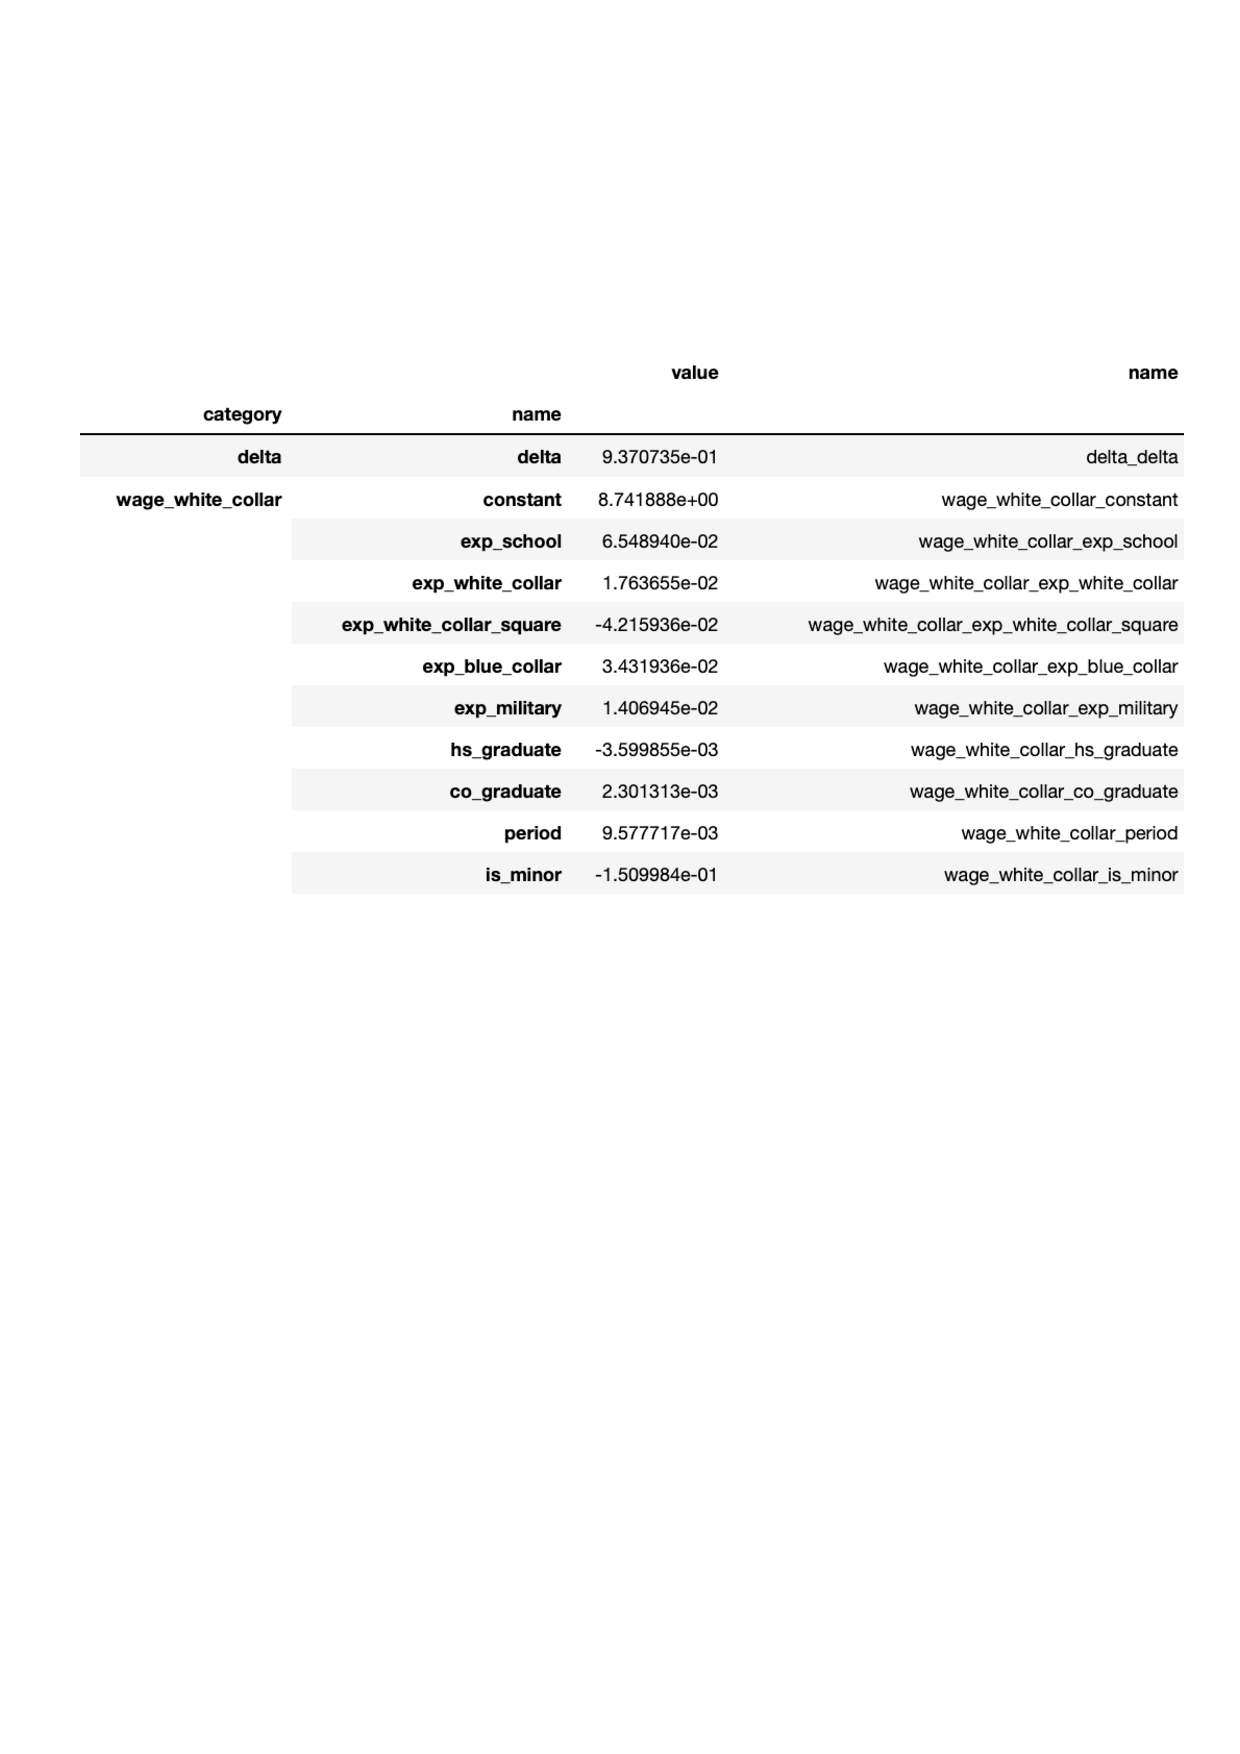
\includegraphics{crop-params.pdf}}}\hspace{0.3cm}
	\subfloat[Options]{\scalebox{0.39}{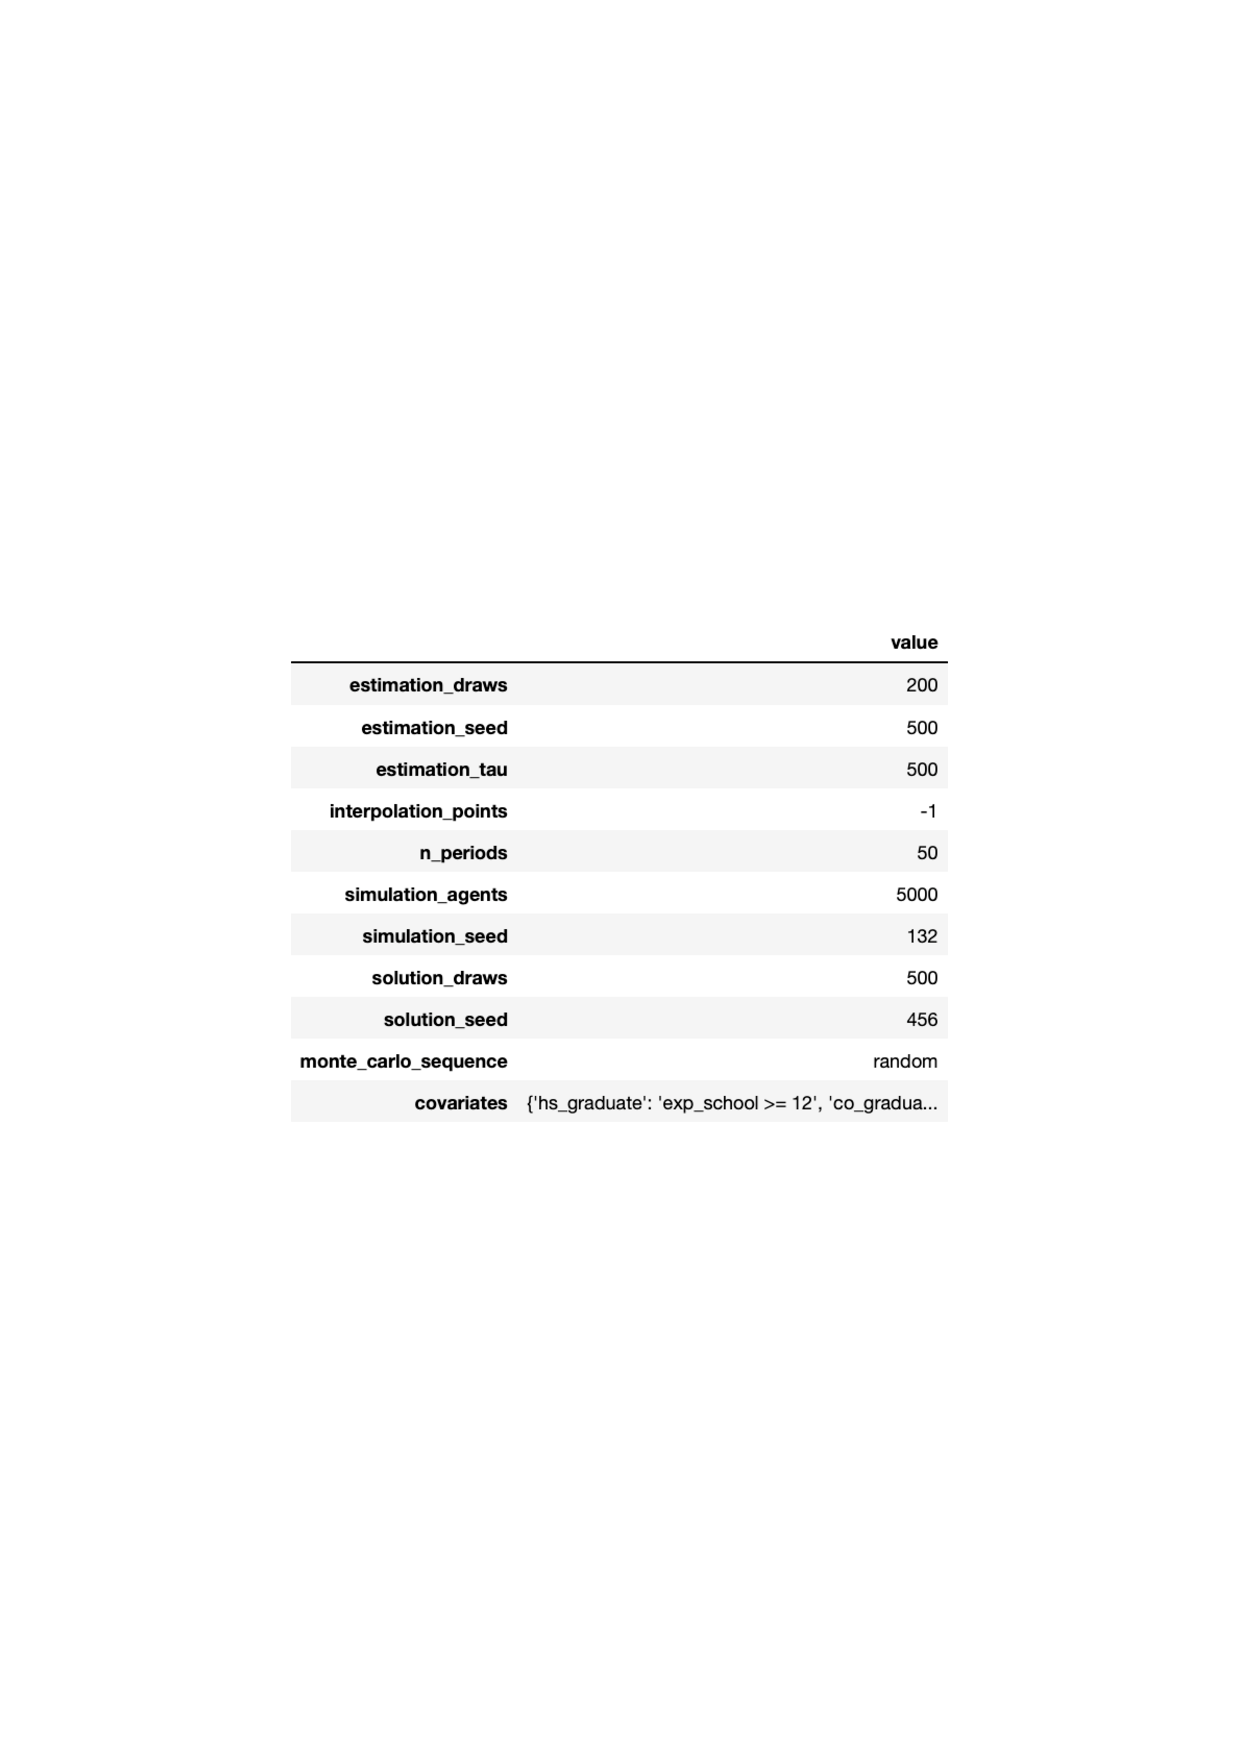
\includegraphics{crop-options.pdf}}}
	\caption{Model specification}\label{Model specification}
\end{figure}%\FloatBarrier

\begin{figure}[b!]\centering
\caption{Dashboard}\label{Dashboard}
\scalebox{0.40}{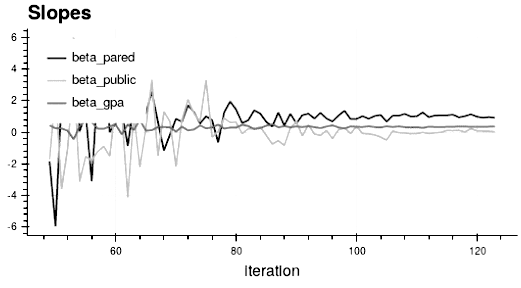
\includegraphics{crop-dashboard-black-white}}
\end{figure}%\FloatBarrier

We adopt a modern software engineering workflow in the development of both packages and tutorials, source code, testing harness, as well as implementation details are available in their respective online documentations at \url{https://respy.rtfd.io} and \url{https://estimagic.rtfd.io}.
